\title{Aula 11 - Criptografia Assimétrica}

\author{Prof. Gabriel Rodrigues Caldas de Aquino}

\institute
{
  Instituto de Computação \\
  Universidade Federal do Rio de Janeiro\\
  gabrielaquino@ic.ufrj.br% Your institution for the title page
}
\date{Compilado em: \\ \today} % Date, can be changed to a custom date

%----------------------------------------------------------------------------------------
%    PRESENTATION SLIDE
%----------------------------------------------------------------------------------------



\begin{frame}
  % Print the title page as the first slide
  \titlepage
\end{frame}

\begin{frame}{Criptografia de Chave Pública}

  A criptografia de chave pública introduz uma mudança fundamental:
  \begin{itemize}
    \item Baseada em \textbf{funções matemáticas}, e não apenas em substituição e permutação.
    \item É \textbf{assimétrica}: utiliza duas chaves separadas (pública e privada), ao contrário da simétrica que usa uma única chave.
    \item Essa assimetria impacta diretamente a \textbf{confidencialidade}, a \textbf{distribuição de chaves} e a \textbf{autenticação}.
    \item Grande parte da teoria dos criptossistemas de chave pública é baseada na teoria dos números.
  \end{itemize}
\end{frame}
\begin{frame}{Criptografia de Chave Pública}

  Concepções equivocadas comuns:
  \begin{itemize}
    \item Não é intrinsecamente mais segura que a criptografia simétrica — a segurança depende do \textbf{tamanho da chave} e do \textbf{custo computacional} para quebrar a cifra.
    \item Não substitui a criptografia simétrica — devido ao \textbf{alto overhead computacional}, continua restrita principalmente a:
          \begin{itemize}
            \item \textbf{Gerenciamento de chaves}
            \item \textbf{Assinaturas digitais}
          \end{itemize}
  \end{itemize}
\end{frame}


\begin{frame}{Criptografia de Chave Pública - Termos comuns}
  \textbf{Chaves Assimétricas}:   Duas chaves relacionadas, uma \textbf{pública} e uma \textbf{privada}, usadas para operações complementares:
  \begin{itemize}
    \item Encriptação e decriptação
    \item Geração e verificação de assinatura
  \end{itemize}


  \textbf{Certificado de Chave Pública}: Documento emitido e assinado digitalmente pela chave privada de uma \textbf{Autoridade de Certificação (CA)}:
  \begin{itemize}
    \item Vincula o \textbf{nome de um assinante} a uma \textbf{chave pública}.
    \item Garante que o assinante identificado tem \textbf{controle exclusivo} da chave privada correspondente.
  \end{itemize}
\end{frame}
\begin{frame}{Criptografia de Chave Pública - Termos comuns}
  \textbf{Algoritmo Criptográfico Assimétrico}: Algoritmo criptográfico que usa duas chaves relacionadas:
  \begin{itemize}
    \item Uma chave \textbf{pública} e uma chave \textbf{privada}.
    \item É computacionalmente inviável derivar a chave privada a partir da pública.
  \end{itemize}


  \textbf{Infraestrutura de Chave Pública (PKI)}: Conjunto de políticas, processos e plataformas para administração de certificados e pares de chaves:
  \begin{itemize}
    \item Emissão, manutenção e revogação de certificados.
    \item Envolve servidores, software e estações de trabalho.
    \item Suporte para autenticação, confidencialidade e integridade.
  \end{itemize}
\end{frame}

\begin{frame}{Como Surgiu a Criptografia Assimétrica}
  O conceito de criptografia de chave pública evoluiu de uma tentativa de atacar \textbf{dois dos problemas mais difíceis associados à encriptação simétrica}:

  \begin{itemize}
    \item  \textbf{A distribuição de chaves} sob a encriptação simétrica:
          \begin{itemize}
            \item  Requer que dois comunicantes já compartilhem uma chave, que de alguma forma foi distribuída a eles; \textbf{OU}
            \item Requer o uso de um centro de distribuição de chaves - Diffie [DIFF88]:
                  “afinal, qual seria a vantagem de desenvolver criptossistemas impenetráveis, se seus usuários fossem forçados a
                  compartilhar suas chaves com um CDC que poderia ser comprometido por roubo ou suborno?”
          \end{itemize}
    \item  \textbf{Assinaturas digitais} - Se o uso da criptografia tivesse que se tornar comum, não apenas nas
          situações militares, mas para fins comerciais e particulares, então as mensagens e documentos eletrônicos precisariam do equivalente das assinaturas usadas nos documentos em papel.
  \end{itemize}
\end{frame}

\begin{frame}{Criptossistemas de chave pública}
  Os algoritmos assimétricos contam com uma chave para encriptação e uma chave diferente, porém relacio  nada, para a decriptação. Eles têm a seguinte característica importante:
  \begin{itemize}
    \item É computacionalmente inviável determinar a chave de decriptação dado apenas o conhecimento do   algoritmo de criptografia e da chave de encriptação.
    \item Além disso, alguns algoritmos, como RSA, também exibem esta característica:  Qualquer uma das duas chaves relacionadas pode ser usada para encriptação, com a outra para a decriptação.
  \end{itemize}


\end{frame}

\begin{frame}{Encriptação com chave pública}

  \begin{figure}
    \centering
    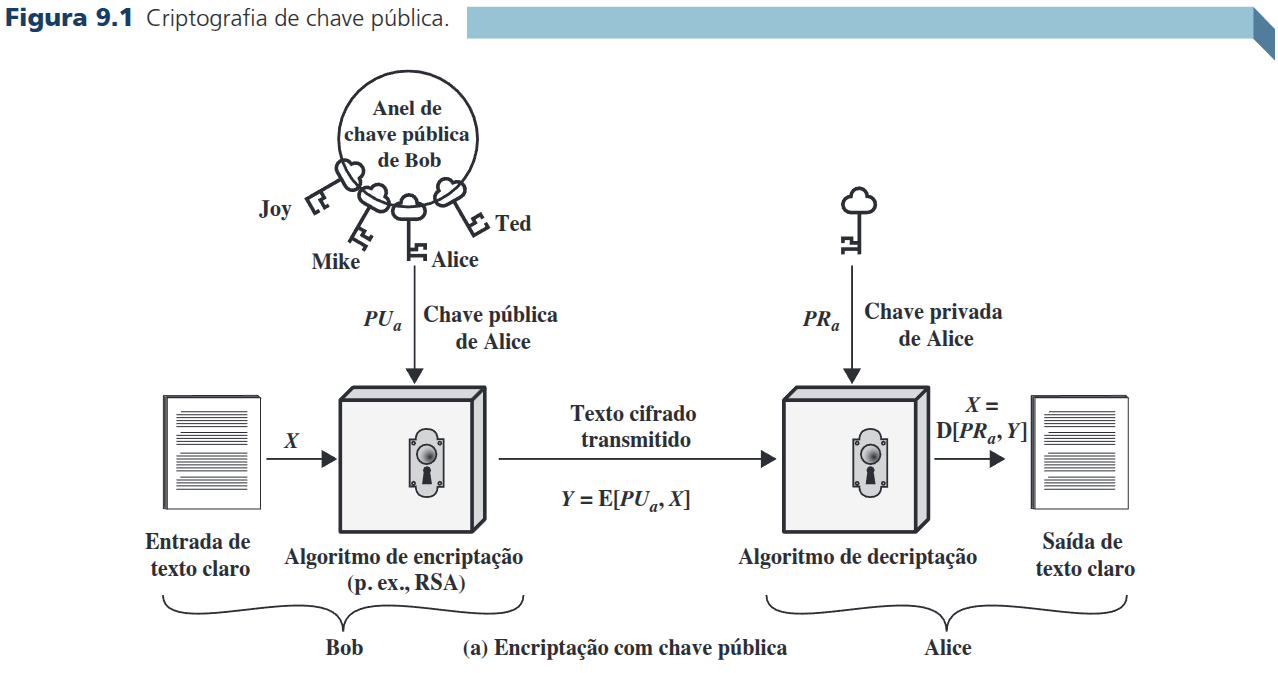
\includegraphics[width=\linewidth]{Figuras/encriptacao-com-chave-publica.png}

  \end{figure}

\end{frame}

\begin{frame}{Encriptação com chave privada}

  \begin{figure}
    \centering
    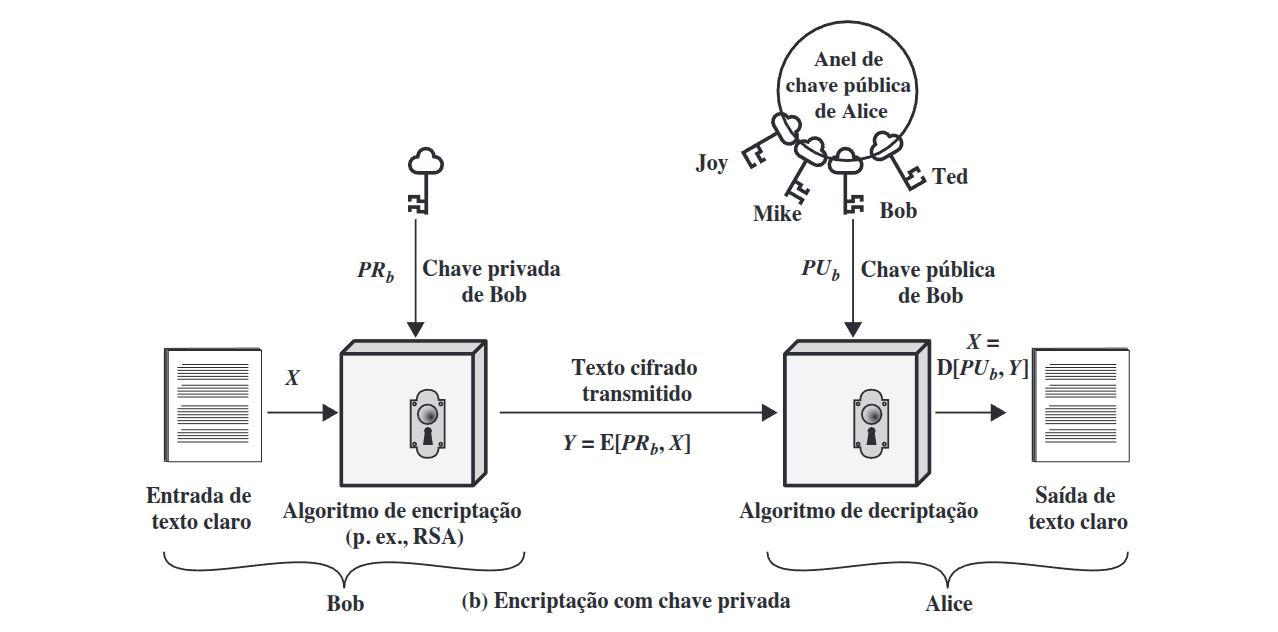
\includegraphics[width=\linewidth]{Figuras/encriptacao-com-chave-privada.png}

  \end{figure}

\end{frame}

\begin{frame}{Etapas Essenciais da Criptografia de Chave Pública}
  \begin{enumerate}
    \item Cada usuário gera um \textbf{par de chaves} (pública e privada) para encriptação e decriptação.
    \item A \textbf{chave pública} é disponibilizada em um repositório ou arquivo acessível; a \textbf{chave privada} permanece secreta.
    \item Para enviar uma mensagem confidencial a Alice, Bob usa a \textbf{chave pública de Alice} para encriptar a mensagem.
    \item Ao receber, Alice utiliza sua \textbf{chave privada} para decriptar. Apenas ela consegue recuperar o texto original.
  \end{enumerate}
\end{frame}


\begin{frame}{Esquema de Encriptação de Chave Pública}
  Um esquema de encriptação de chave pública possui cinco elementos principais:
  \begin{enumerate}
    \item \textbf{Texto claro}: mensagem ou dados legíveis fornecidos como entrada.
    \item \textbf{Algoritmo de encriptação}: aplica transformações no texto claro.
    \item \textbf{Chaves pública e privada}: par de chaves; se uma encripta, a outra decripta.
    \item \textbf{Texto cifrado}: mensagem embaralhada gerada como saída, dependente da chave.
    \item \textbf{Algoritmo de decriptação}: reverte o processo, recuperando o texto claro original.
  \end{enumerate}
\end{frame}

\begin{frame}{Criptossitema de chave pública - Objetivo Sigilo}

  \begin{figure}
    \centering
    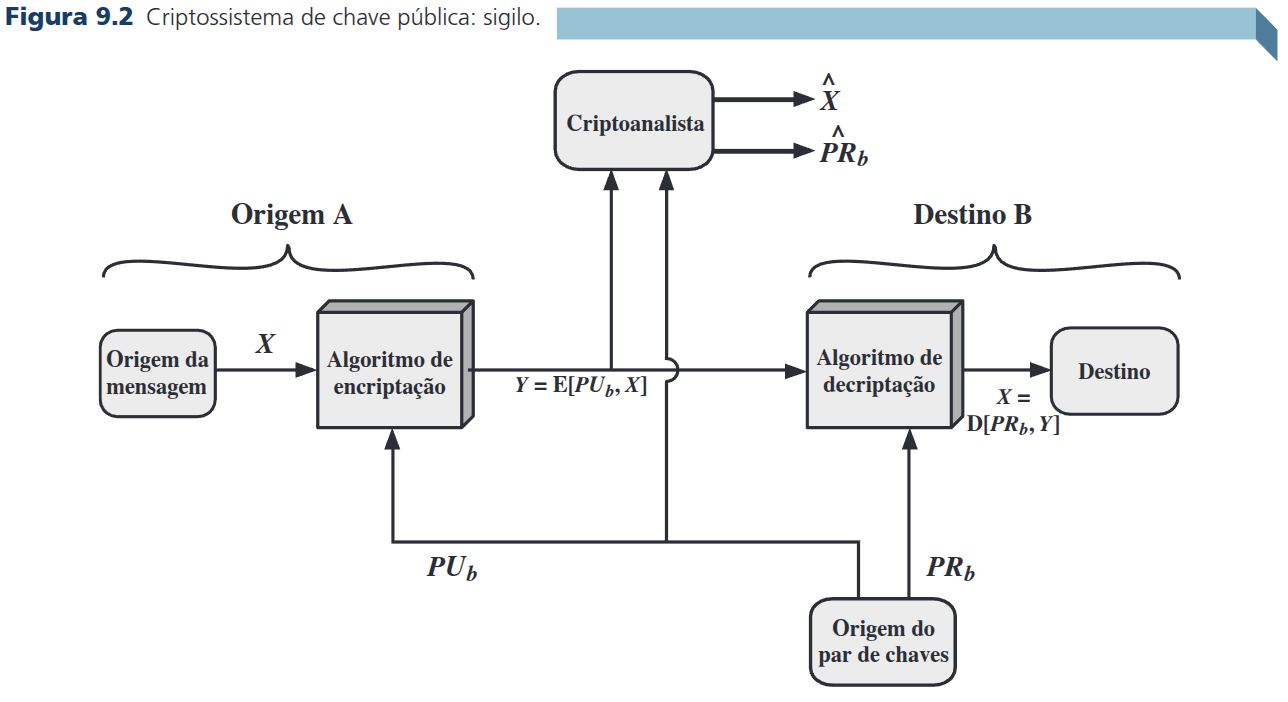
\includegraphics[width=\linewidth]{Figuras/criptossistema-chave-publica.png}

  \end{figure}

\end{frame}

\begin{frame}{Criptossitema de chave pública - Objetivo autenticação}

  \begin{figure}
    \centering
    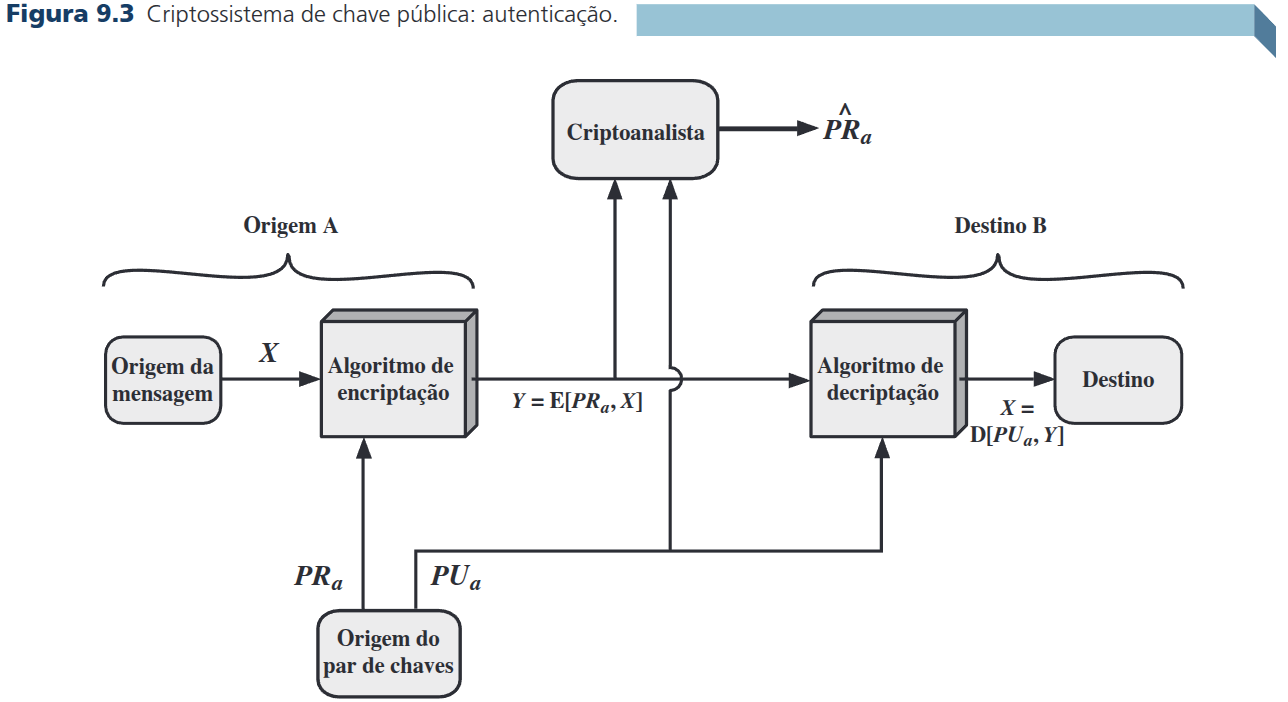
\includegraphics[width=0.9\linewidth]{Figuras/criptossistema-chave-publica-autenticacao.png}

  \end{figure}

\end{frame}

\begin{frame}{Autenticação e Confidencialidade com Chave Pública}
  \textbf{Importante}:
  \begin{itemize}
    \item Apenas a encriptação com a chave privada do emissor garante \textbf{autenticação}, mas não a confidencialidade.
    \item Para prover \textbf{ambos}, aplica-se uma dupla encriptação:
  \end{itemize}

  \[
    Z = E(PU_b, \; E(PR_a, \; X))
  \]
  \[
    X = D(PU_a, \; D(PR_b, \; Z))
  \]

  \begin{itemize}
    \item O emissor primeiro encripta com sua \textbf{chave privada} (assinatura digital).
    \item Em seguida, encripta novamente com a \textbf{chave pública do receptor}.
    \item O receptor, ao decriptar, recupera tanto a \textbf{confidencialidade} quanto a \textbf{autenticidade}.
    \item Desvantagem: exige 4 operações de criptografia assimétrica por mensagem.
  \end{itemize}
\end{frame}

\begin{frame}{Criptossitema de chave pública - Objetivo autenticação e sigilo}

  \begin{figure}
    \centering
    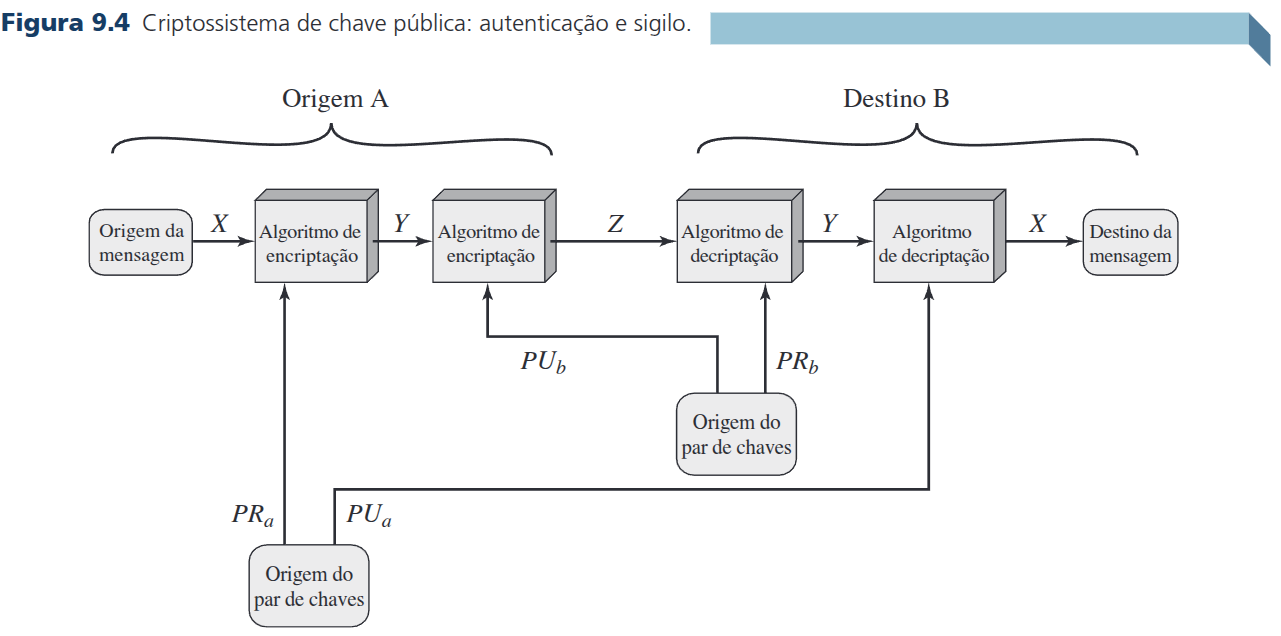
\includegraphics[width=\linewidth]{Figuras/criptossistema-de-chave-publica-autenticacao-e-sigilo.png}

  \end{figure}

\end{frame}

\begin{frame}{Aplicações de criptografia de chave pública}

  \begin{figure}
    \centering
    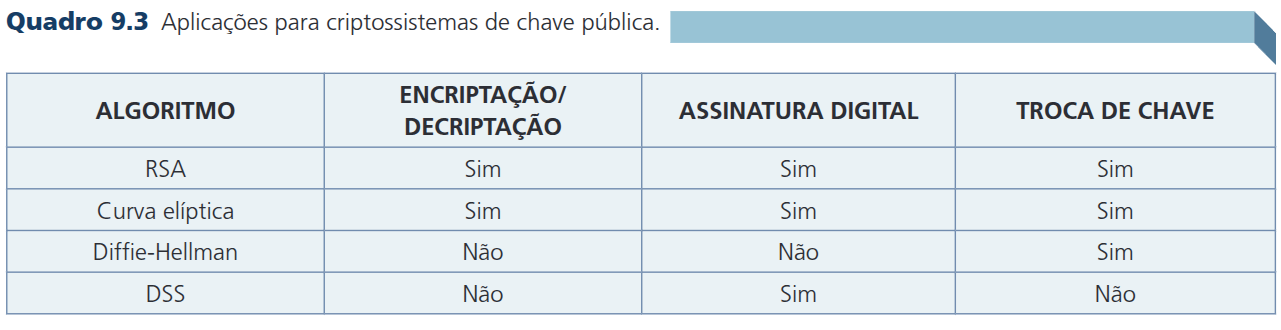
\includegraphics[width=\linewidth]{Figuras/aplicacoes-criptografia-chave-publica.png}

  \end{figure}
  \textbf{Obs}: DSS é a sigla para
  Digital Signature Standard, um padrão de assinatura digital que, em conjunto com o DSA (Digital Signature Algorithm) e o SHA (Secure Hash Algorithm), permite a criação de assinaturas digitais e verificação de integridade de dados, utilizando criptografia de chave pública de forma a garantir a autenticidade e a não-repudiação de uma transação
\end{frame}

\begin{frame}{Requisitos para Criptografia de Chave Pública}
  \begin{enumerate}
    \item Geração de par de chaves $(PU_b, PR_b)$ deve ser \textbf{computacionalmente fácil}.
    \item Encriptação: dado $PU_b$ e $M$, calcular $C = E(PU_b, M)$ deve ser \textbf{fácil}.
    \item Decriptação: dado $PR_b$ e $C$, calcular $M = D(PR_b, C)$ deve ser \textbf{fácil}.
    \item \textbf{Inviável} obter $PR_b$ a partir de $PU_b$.
    \item \textbf{Inviável} recuperar $M$ conhecendo apenas $PU_b$ e $C$.
    \item (Opcional) Ordem das chaves pode ser invertida:
          $M = D[PU_b, E(PR_b, M)] = D[PR_b, E(PU_b, M)]$.
  \end{enumerate}

  \vspace{0.3cm}
  \textbf{Observação:} Apenas poucos algoritmos atendem a todos os requisitos, como RSA, ECC, Diffie-Hellman e DSS.
\end{frame}
\begin{frame}{Função de Mão Única com Alçapão}
  \begin{itemize}
    \item Função de mão única: mapeia um domínio $X$ em um intervalo $Y$ de forma que:
          \[
            Y = f(X) \text{ é fácil de calcular, mas } X = f^{-1}(Y) \text{ é inviável de obter.}
          \]
    \item "Com alçapão": existe uma informação secreta que permite inverter a função de forma eficiente.
    \item Essencial para criptografia de chave pública: permite encriptação segura sem compartilhar a chave privada.
  \end{itemize}

\end{frame}

\begin{frame}{Complexidade de Funções Criptográficas}
  \begin{itemize}
    \item \textbf{Fácil}: problema resolvível em tempo polinomial $O(n^a)$ em função do tamanho da entrada $n$. Onde $a$ é uma constante fixa.
    \item Algoritmos polinomiais pertencem à classe P.
    \item \textbf{Inviável}: problema cujo esforço cresce mais rápido que o tempo polinomial, por exemplo, $O(2^n)$.
    \item Observação: medir complexidade pelo pior caso ou caso médio não é suficiente para criptografia.
    \item Criptografia exige que a função seja inviável de reverter para \textbf{praticamente todas as entradas}.
  \end{itemize}
\end{frame}
\begin{frame}{Função de Mão Única com Alçapão}
  \begin{itemize}
    \item Uma função que é fácil de calcular em uma direção e inviável na outra, a menos que informação adicional (alçapão) seja conhecida.
    \item Formalmente, uma família de funções reversíveis $f_k$:
          \begin{itemize}
            \item $Y = f_k(X)$ é fácil, se $k$ e $X$ forem conhecidos.
            \item $X = f_k^{-1}(Y)$ é fácil, se $k$ e $Y$ forem conhecidos.
            \item $X = f_k^{-1}(Y)$ é inviável, se apenas $Y$ for conhecido, sem $k$.
          \end{itemize}
    \item A construção de esquemas de \textbf{chave pública} depende de \textbf{encontrar funções de mão única com alçapão adequadas}.
  \end{itemize}
\end{frame}

\begin{frame}{Algoritmo RSA}
  \begin{itemize}
    \item O artigo de Diffie e Hellman (1976) desafiou a comunidade a criar algoritmos de chave pública. \href{https://dl.acm.org/doi/10.1145/1499799.1499815}{\textcolor{blue}{Referência}}
    \item Muitos algoritmos iniciais se mostraram falhos.
    \item Em 1977, Ron Rivest, Adi Shamir e Len Adleman (MIT) desenvolveram o esquema RSA. \href{https://dl.acm.org/doi/10.1145/359340.359342}{\textcolor{blue}{Referência}}
    \item Publicado em 1978, o RSA se tornou a técnica mais aceita e amplamente implementada para criptografia de chave pública.
  \end{itemize}
\end{frame}
\begin{frame}{Funcionamento do RSA}
  \begin{itemize}
    \item RSA é uma cifra de bloco: texto claro e cifrado são inteiros entre 0 e $n-1$.
    \item Tamanho típico: $n \approx 1024$ bits (309 dígitos decimais).
    \item Cada bloco de texto claro $M$ deve satisfazer $0 \le M < n$.
    \item Encriptação e decriptação:
          \[
            C = M^e \mod n,
          \]
          \[
            \quad M = C^d \mod n = (M^e)^d \mod n
          \]
    \item Chave pública: $PU = \{e, n\}$
          Chave privada: $PR = \{d, n\}$
    \item Requisitos:
          \begin{enumerate}
            \item $M^{ed} \mod n = M$ para todo $M < n$
            \item Calcular $M^e \mod n$ e $C^d \mod n$ é relativamente fácil
            \item Conhecendo $e$ e $n$, é inviável determinar $d$
          \end{enumerate}
    \item $d$ pode ser calculado usando o algoritmo de Euclides estendido
  \end{itemize}
\end{frame}
\begin{frame}{Requisito de Inversão no RSA}
  \begin{itemize}
    \item Para garantir $M^{ed} \mod n = M$, os expoentes $e$ e $d$ devem ser inversos multiplicativos módulo $\varphi(n)$, onde $\varphi(n)$ é a função totiente de Euler.
    \item Para $n = pq$, com $p$ e $q$ primos:
          \[
            \varphi(n) = (p-1)(q-1)
          \]
    \item Relação entre $e$ e $d$:
          \[
            ed \equiv 1 \mod \varphi(n) \quad \Rightarrow \quad d \equiv e^{-1} \mod \varphi(n)
          \]
    \item Condição: $e$ e $d$ devem ser relativamente primos a $\varphi(n)$:
          \[
            \gcd(d, \varphi(n)) = 1
          \]
  \end{itemize}

\end{frame}

\begin{frame}{Inverso Multiplicativo no RSA}
  No RSA, a chave privada $d$ é escolhida como o inverso multiplicativo de $e$ módulo $\varphi(n)$:

  \[
    d \equiv e^{-1} \pmod{\varphi(n)}
  \]

  \begin{itemize}
    \item Isso significa que $d$ satisfaz:
          \[
            d \cdot e \equiv 1 \pmod{\varphi(n)}
          \]
    \item Exemplo: $e = 7$, $\varphi(n) = 160$
          \[
            23 \cdot 7 = 161 \equiv 1 \pmod{160}
          \]
    \item Portanto, $d = 23$ é o inverso multiplicativo de $e = 7$ módulo 160.

  \end{itemize}
\end{frame}


\begin{frame}{Esquema RSA}
  \textbf{Ingredientes:}
  \begin{itemize}
    \item Dois números primos secretos: $p$ e $q$.
    \item Calcula-se $n = pq$ (público).
    \item Escolhe-se $e$ tal que $mdc(\varphi(n), e) = 1$ e $1 < e < \varphi(n)$ (público).
    \item Calcula-se $d \equiv e^{-1} \mod \varphi(n)$ (privado).
  \end{itemize}

  \textbf{Chaves:}
  \begin{itemize}
    \item Chave privada: $\{d, n\}$
    \item Chave pública: $\{e, n\}$
  \end{itemize}

  \textbf{Processo de encriptação e decriptação:}
  \begin{itemize}
    \item Usuário B quer enviar mensagem $M$ para A:
          \[
            C = M^e \mod n \quad \text{(encriptação)}
          \]
    \item Usuário A recebe $C$ e decripta:
          \[
            M = C^d \mod n
          \]
  \end{itemize}
\end{frame}
\begin{frame}{Tabela resumo dos parâmetros do RSA}

  \begin{figure}
    \centering
    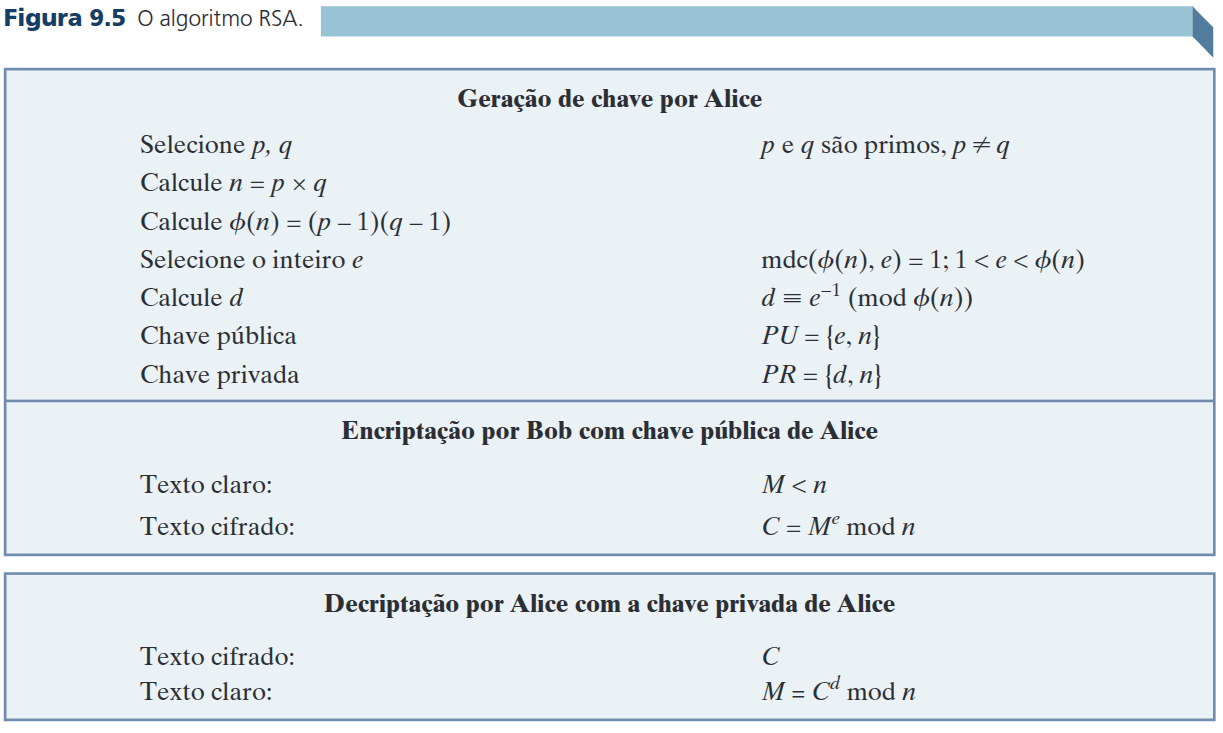
\includegraphics[width=0.8\linewidth]{Figuras/tabela-resumo-rsa.png}

  \end{figure}

\end{frame}
\begin{frame}{Exemplo Numérico do RSA}
  \textbf{Geração de chaves:}
  \begin{itemize}
    \item $p = 17$, $q = 11$
    \item $n = pq = 187$
    \item $\varphi(n) = (p-1)(q-1) = 160$
    \item Escolhe $e = 7$, $mdc(e, 160) = 1$
    \item Calcula $d \equiv e^{-1} \mod 160 \Rightarrow d = 23$
  \end{itemize}

  \begin{block}{Explicação}
    \begin{itemize}
      \item Exemplo: $e = 7$, $\varphi(n) = 160$
            \[
              23 \cdot 7 = 161 \equiv 1 \pmod{160}
            \]
      \item Portanto, $d = 23$ é o inverso multiplicativo de $e = 7$ módulo 160.

    \end{itemize}

  \end{block}

  \textbf{Chaves:}
  \begin{itemize}
    \item Pública: $PU = \{7, 187\}$
    \item Privada: $PR = \{23, 187\}$
  \end{itemize}
\end{frame}
\begin{frame}{Exemplo Numérico do RSA}
  \textbf{Encriptação de $M = 88$:}
  \[
    C = M^e \mod n = 88^7 \mod 187
  \]
  \[
    88^7 \mod 187 = (88 \times 88^2 \times 88^4) \mod 187 = (88 \times 77 \times 132) \mod 187 = 11
  \]

  \textbf{Decriptação:}
  \[
    M = C^d \mod n = 11^{23} \mod 187
  \]
  \[
    11^{23} \mod 187 = 88
  \]

  \textbf{Resultado:} A mensagem original $M = 88$ é recuperada com sucesso.
\end{frame}
\begin{frame}{Exemplo Simples numérico - RSA}

  \begin{figure}
    \centering
    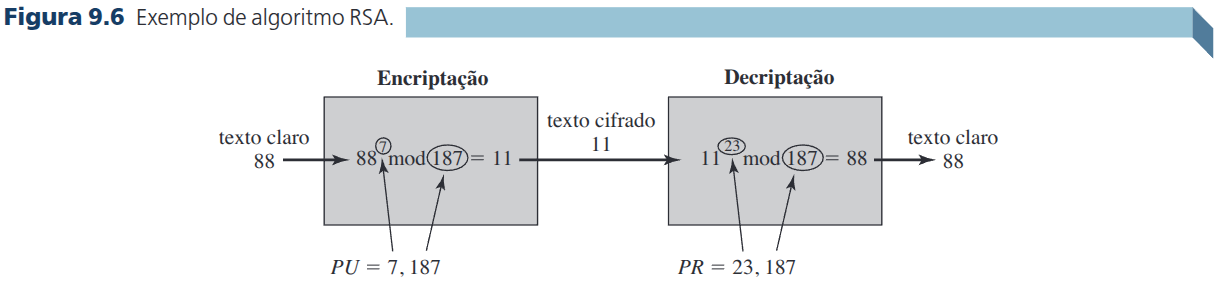
\includegraphics[width=\linewidth]{Figuras/exemplo-rsa-numerico-simples.png}

  \end{figure}

\end{frame}

\begin{frame}{Processamento de múltiplos blocos usando RSA}

  \begin{figure}
    \centering
    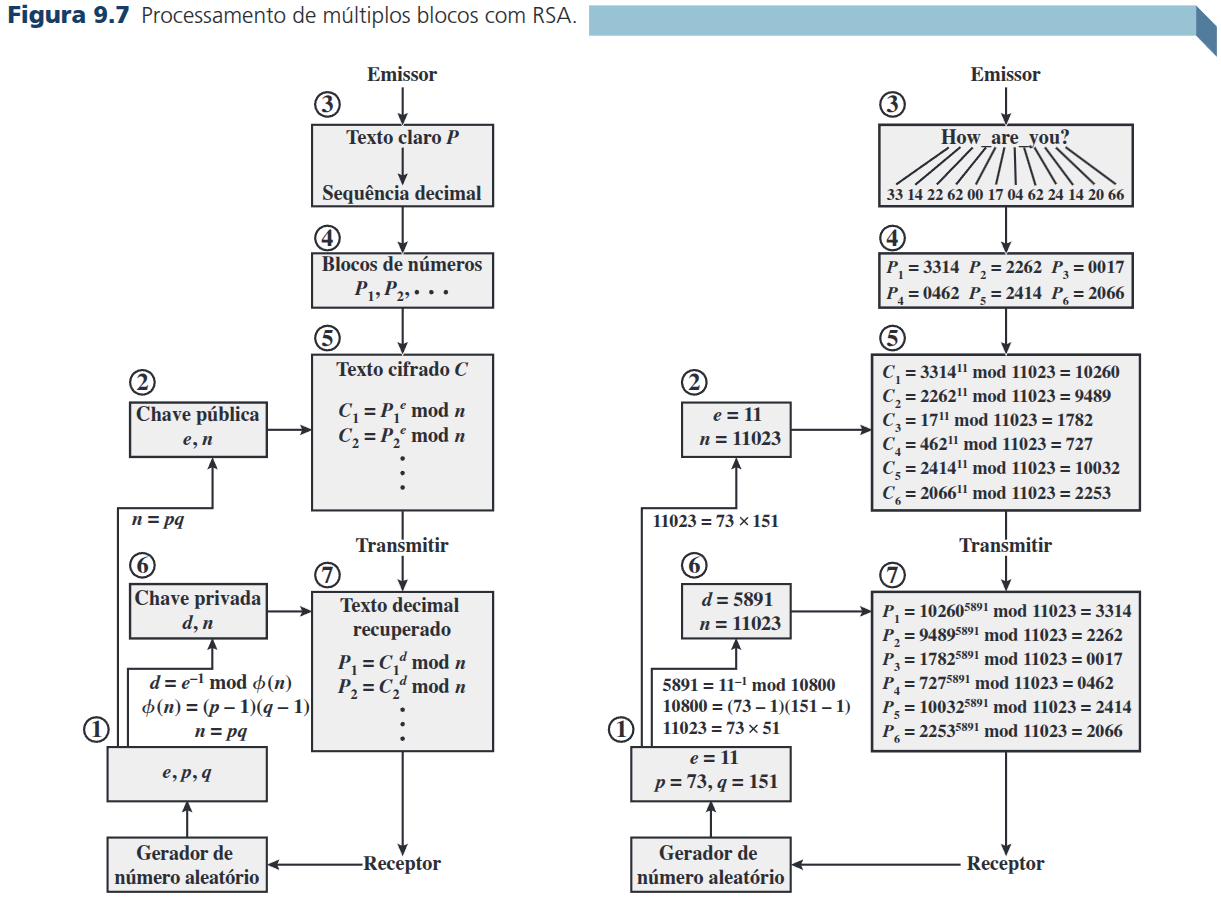
\includegraphics[width=0.7\linewidth]{Figuras/processamento-multiplos-blocos-rsa.png}

  \end{figure}

\end{frame}